\documentclass[a4paper,11pt]{article}
\usepackage[utf8]{inputenc}
\usepackage{amsmath}
\usepackage{amsfonts}
\usepackage{amssymb}
\usepackage{graphicx}
\usepackage[backend=biber]{biblatex}

\addbibresource{nn.bib}
\renewcommand\thesubsection{\alph{subsection}}


%opening
\title{Delay-dependent synchronized firing in neural columns}
\author{Vince Baker, advisor: Dr. Luis Cruz Cruz\\ Drexel University Department of Physics}

\begin{document}

\maketitle

\begin{abstract}
We demonstrate that neuron firings in a column structure can become synchronized when the actional potential propagation time between neurons depends on the inter-neuron distance.

\end{abstract}

\section{Introduction} 
Synchronization in networks of neurons may arise from a combination of the network topology, interaction strengths, stimulus properties and neuron and synapse dynamics.

\section{Methods}
We simulated the dynamics of a small neural column to explore neuron synchronization.
Our network geometry is based on the model presented in \cite{markram1998}.
The neural column is composed of 135 neurons on a unit column, 3x3 neurons wide and 9 neurons high as shown in figure \ref{fig:column_structure}.
The neurons are connected according to a distance-based rule:
\begin{align}\label{eq:connectivity}
 P_{a,b} &= C \times e^{-(D(a,b)/\lambda)^2}
\end{align}
We model the neurons using the Izhikevich model \cite{izhikevich2003} to allow us to explore the neural dynamics.
The Izhikevich model uses two coupled differential equations with two variables and four parameters:
\begin{align}
 v^\prime &= 0.04v^2+5v+140-u+I\\
 u^\prime &= a(bv-u)\\
 \text{if } &v>30: v\leftarrow c, u\leftarrow u+d
\end{align}
This is a simplified model of a two-dimensional dynamical system.
This model has been used to reproduce common neural firing patterns.
There is MATLAB code available that implements this neural model with fixed, single-time-step action potential propagation.
\\
We enhanced the available MATLAB code for the Izhikevich model to incorporate propagation time between the neurons through the use of a delay buffer.
This allowed us to study the temporal effects of action potential propagation times.
We simulate networks with both random propagation delays and propagation delays that depend on the distance between the neurons.
\\
There are a number of ways to characterize the degree of synchronization in a network.
One simple measure of spike train synchronization is the correlation between the spike trains.
Improved distance metrics have been developed that are timescale-independent and time-resolved including inter-spike interval (ISI) and SPIKE \cite{kreuz2012}.
The SPIKE metric in particular provides an improved time-resolved distance metric across time scales and time shifts.
\section{Results}
We explored the effect of our distance-dependent propagation times on the dynamics of a neural column.
To test the effect of the distance-dependent propagation times we created two columns, 3x3x40,  with identical neurons and identical connectivity. \\
\begin{figure}[ht]
 \caption{Column structure used in this research, $\lambda=2$,$C=1$,}
 \label{fig:column_structure}
 \centering
   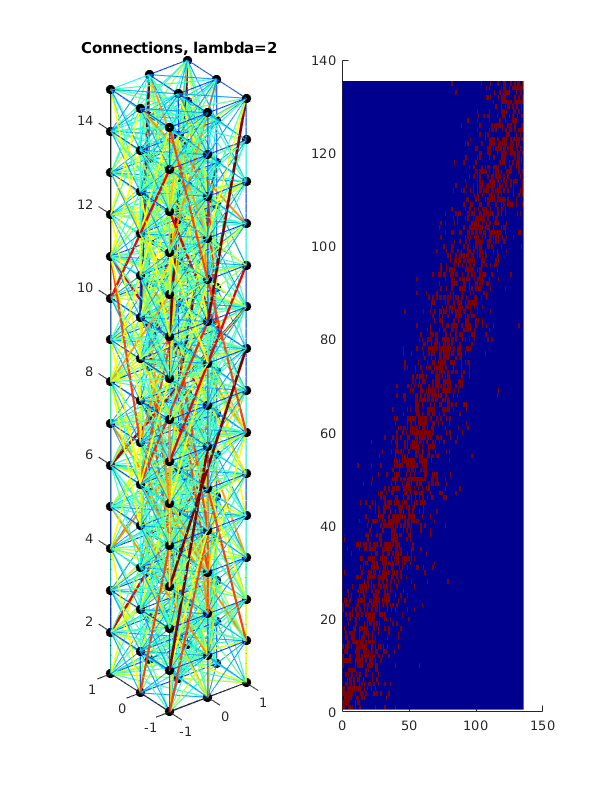
\includegraphics[width=0.48\textwidth]{fig/lambda2}
\end{figure}
The first column has random propagation times, the second column uses distance-dependent propagation times.
The bottom 10 layers were stimulated with the random thalamic input as described in \cite{izhikevich2003}.
The resulting firing patterns are shown in figure \ref{fig:delaycompare}. \\
\begin{figure}[ht]
 \caption{Two identical neural columns, 3x3x40, with randomized propagation delays (top) and distance-dependent propagation delays (bottom) were stimulated with random input in the first 10 layers,
 The column with distance-dependent propagation delays shows synchronized firing that induce traveling wave packets through the column.}
 \label{fig:delaycompare}
 \centering
   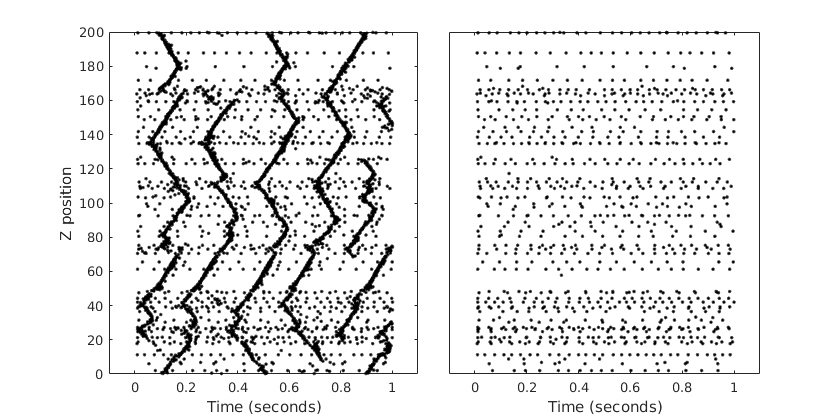
\includegraphics[width=\textwidth]{fig/DelayCompare_RandInput}
\end{figure}
The column with random delay shows random firing activity in the stimulated region, but no propagation through the column.
The column with distance-dependent propagation shows correlated firings with a clear propagation down the column.
These results demonstrate that distance-dependent propagation delay can be a critical parameter in the qualitative behavior of a neural circuit.\\
We also simulated ensembles of column structures as shown in \ref{fig:column_ensemble}.
\begin{figure}[ht]
 \caption{Column ensemble with four columns}
 \label{fig:column_ensemble}
 \centering
   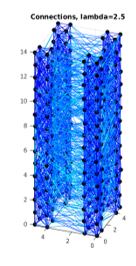
\includegraphics[width=0.48\textwidth]{fig/multicolumn}
\end{figure}
The ensembles were constructed from 2x2 columns that were physically separated by three units. 
The distance-based metric was used to create the ensemble connectivity, resulting in stronger connectivity within columns with weak connectivity between columns.
The first column ensemble was constructed with random propagation times, the second column ensemble with distance-dependent propagation times.
The neuron parameters, connectivity, and stimulus are identical for both ensembles.
The bottom 10 layers of each column ensemble was stimulated with thalamic input.
We again see synchronized firing emerge from the ensemble with distance-dependent propagation delay.
\begin{figure}[ht]
 \caption{Two identical neural columns ensembles with randomized propagation delays (top) and distance-dependent propagation delays (bottom) were stimulated with random input in the first 10 layers,
 The ensemble with distance-dependent propagation delays shows synchronized firing that induce traveling wave packets through the ensemble.}
 \label{fig:delaycompare_column}
 \centering
   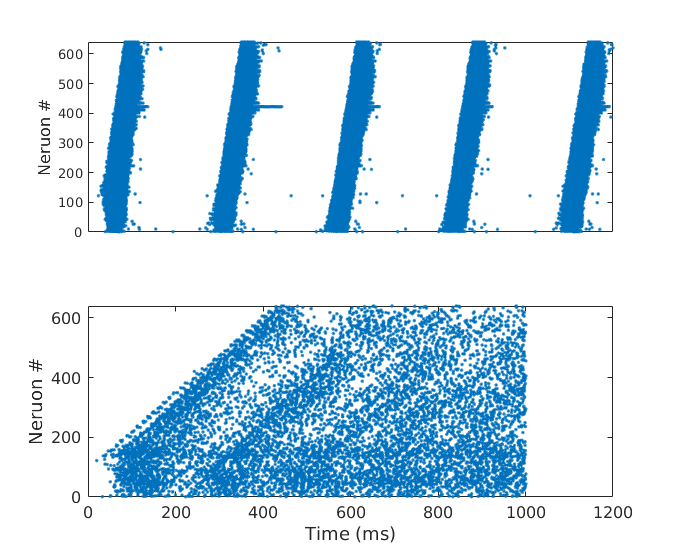
\includegraphics[width=\textwidth]{fig/DelayCompare_ColumnEnsemble}
\end{figure}
\\
The wave propagation phenomenon is particularly interesting in the context of \cite{keane2015} where similar propagating waves arose from random input in a two-dimensional neural circuit.
The authors in \cite{keane2015} propose these propagating waves as a mechanism for synchronizing a network of fundamentally irregular neurons. 

\section{Future work}


\clearpage
\printbibliography

\end{document}
